%% Aktuelle Situation des Arbeitsmarktes
% Ausblick auf das Fehlen von Arbeitskräften
Das Freizügigkeitsabkommen zwischen der Schweiz und der EU regelt die Bedingungen für den freien
Personenverkehr. Damit erhalten Staatsangehörige der Schweiz und der EU das Recht, ihren Arbeitsplatz sowie
ihren Aufenthaltsort innerhalb der Vertragsparteien frei zu wählen. Einzige Voraussetzungen sind, dass sie über 
eine Krankenversicherung, einen nachweisbaren Erwerb (selbstständig oder mit gültigem Arbeitsvertrag) oder über 
genügend finanzielle Mittel für einen dauerhaften Aufenthalt verfügen \cite[S. 1]{ADMIN:PF}. Das Schweizer Parlament 
hat zudem mehrere flankierende Massnahmen beschlossen, um Sozialmissbrauch und Lohndumping zu erschweren \cite[S. 5-6]{ADMIN:PF}.
Als Folge der Einführung der Personenfreizügigkeit im Jahr 2001 und des wirtschaftlichen Erfolgs der Schweiz hat die 
Zuwanderung aus der EU erheblich zugenommen. Insbesondere kurz vor der globalen 
Finanzkrise als der Wirtschaftsmotor auf hochtouren lief, war der Bedarf an zusätzlichen Arbeitskräften immens, was zu einer hohen 
Zuwanderung führte (Abb.~\ref{fig:zuwanderungsaldi}). Dabei sind die Zuwanderer keine Sozialschmarozer, wie es von der SVP heisst, 
sondern mehrheitlich hochqualifizierte Arbeitskräfte. Tatsächlich übersteigt das durchschnittliche Bildungsniveau der Zuwanderer
jenes der bereits ansässigen Wohnbevölkerung deutlich \cite[S. 5-6]{ADMIN:Bericht}. Dadurch ist der Anteil der Erwerbstätigkeit bei
Zuwanderern aus dem EU-Raum im Jahr 2010 auf das gleiche hohe Niveau (84\%) der Schweizer gestiegen. Durch diese hohe Erwärbstätigkeit 
und die damit verbundene Kaufkraft hat die Zuwanderung während der ganzen Wirtschaftskrise den inländischen Konsum und die
Bauinvestitionen gestützt. Die Binnenwirtschaft der Schweiz konnte die Krise somit erheblich besser als die
europäischen Nachbarn überstehen und bereits früh wieder in eine Wachstumsphase übergehen. Durch das stabile Wachstum der Schweiz in der 
Vergangenheit und die konjunkturelle Erholung der Weltwirtschaft wird der Schweizer Arbeitsmarkt ein weiteres Wachstum erleben. Es existieren Prognosen, 
welche davon ausgehen, dass trotz der Zuwanderung bis ins Jahr 2030 etwa 400'000 Arbeitnehmer fehlen werden \cite[S. 4]{BASS:Arbeitskraeftemangel}.
Der Schweizer Arbeitsmarkt ist also heute wie auch in Zukunft sehr aufnahmefähig. Durch diesen Anstieg der Beschäftigung werden die Einkommen
der Sozialversicherungen steigen und so deren Stabilität gewährleisten.
\newpage

\begin{figure*}[h]
	\begin{center}
		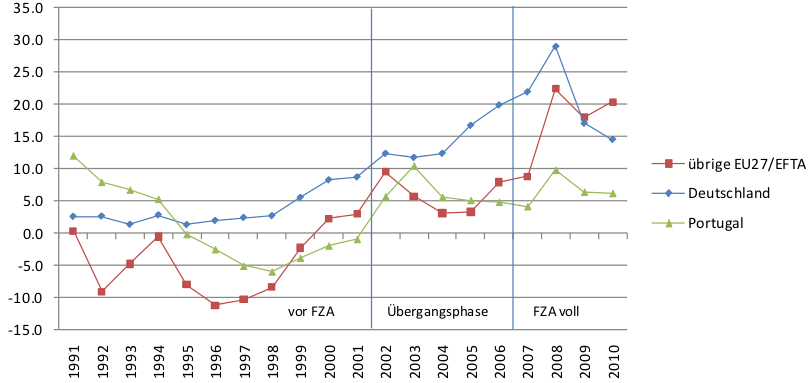
\includegraphics[width=0.9\textwidth]{images/Zuwanderungssaldo_Bericht_2.png}
	\end{center}
	\caption{Verlauf der Zuwanderung nach Herkunftsländern in Tausend \cite[S. 18]{ADMIN:Bericht}}
	\label{fig:zuwanderungsaldi}
\end{figure*}

